% Include from the project root; requires \usepackage{graphicx}.
\begin{figure*}[t]
  \centering
  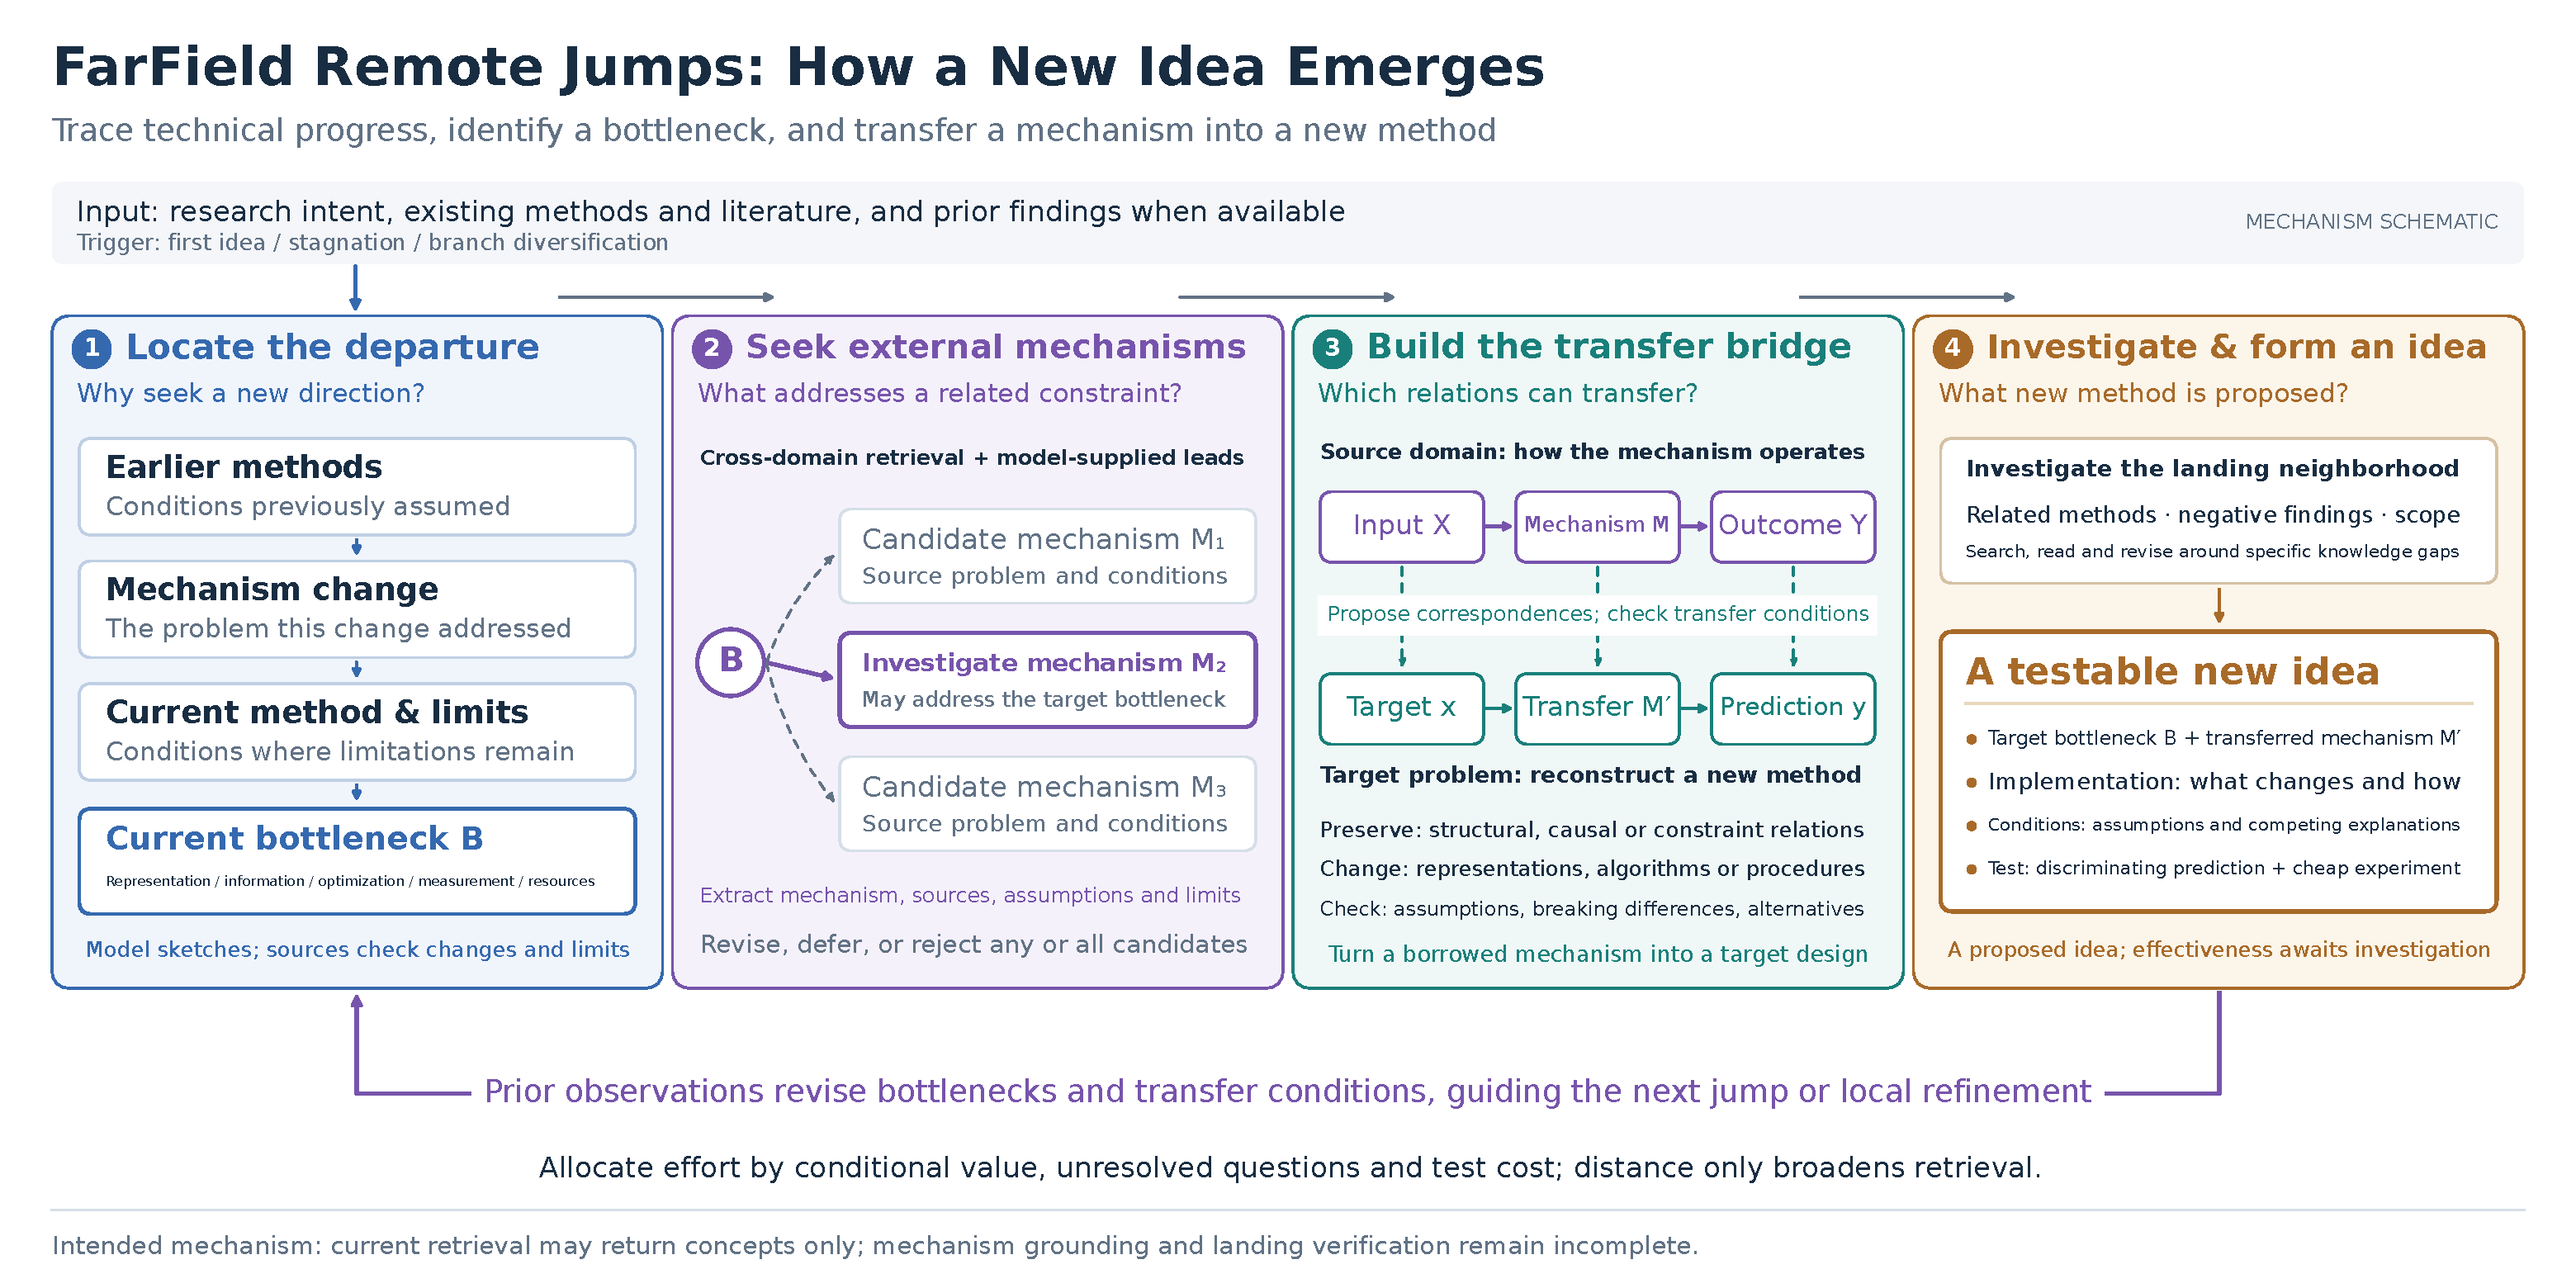
\includegraphics[width=\textwidth]{figures/farfield_remote_jump_en.pdf}
  \caption{Idea formation through the intended FarField remote-jump mechanism.
  Technical history and prior findings identify a target bottleneck.
  Cross-domain retrieval and model-supplied leads expose candidate mechanisms.
  A proposed transfer maps source relationships to a target design while
  making assumptions, breaking differences, and competing explanations explicit.
  Inquiry into the landing neighborhood revises the design into a testable
  idea with a concrete implementation change and a discriminating experiment.
  Candidate emphasis denotes inquiry priority, not verified effectiveness;
  dashed correspondences are proposed mappings to be checked.
  Subsequent observations guide later jumps or local refinement.
  This is a mechanism schematic, not a complete system architecture or evidence
  that mechanism grounding and landing verification are already reliable.}
  \label{fig:farfield-remote-jump}
\end{figure*}
